O firmwawe para o aeropêndulo foi desenvolvido a partir de bibliotecas, cada biblioteca tem sua funcionalidade, com isso o projeto se torna mais flexível, podendo ser atualizado e incrementado a medida que o projeto se torne mais robusto. 

Para desenvolver o firmware, utilizamos a ferramenta de plataforma cruzada PlatformIO. Essa ferramenta foi criada com o propósito de centralizar o desenvolvimento de firmware, possibilitando a programação para diversos microcontroladores, como o ESP32, a Família do Arduino, STM32 e muitos outros. Isso torna o projeto ainda mais flexível e versátil. A arquitetura é descrita na Figura \ref{fig3:image_16}.


\begin{figure}[!h]
	\centering
	\caption{Arquitetura do Firmware do Aeropêndulo.}
	\efbox{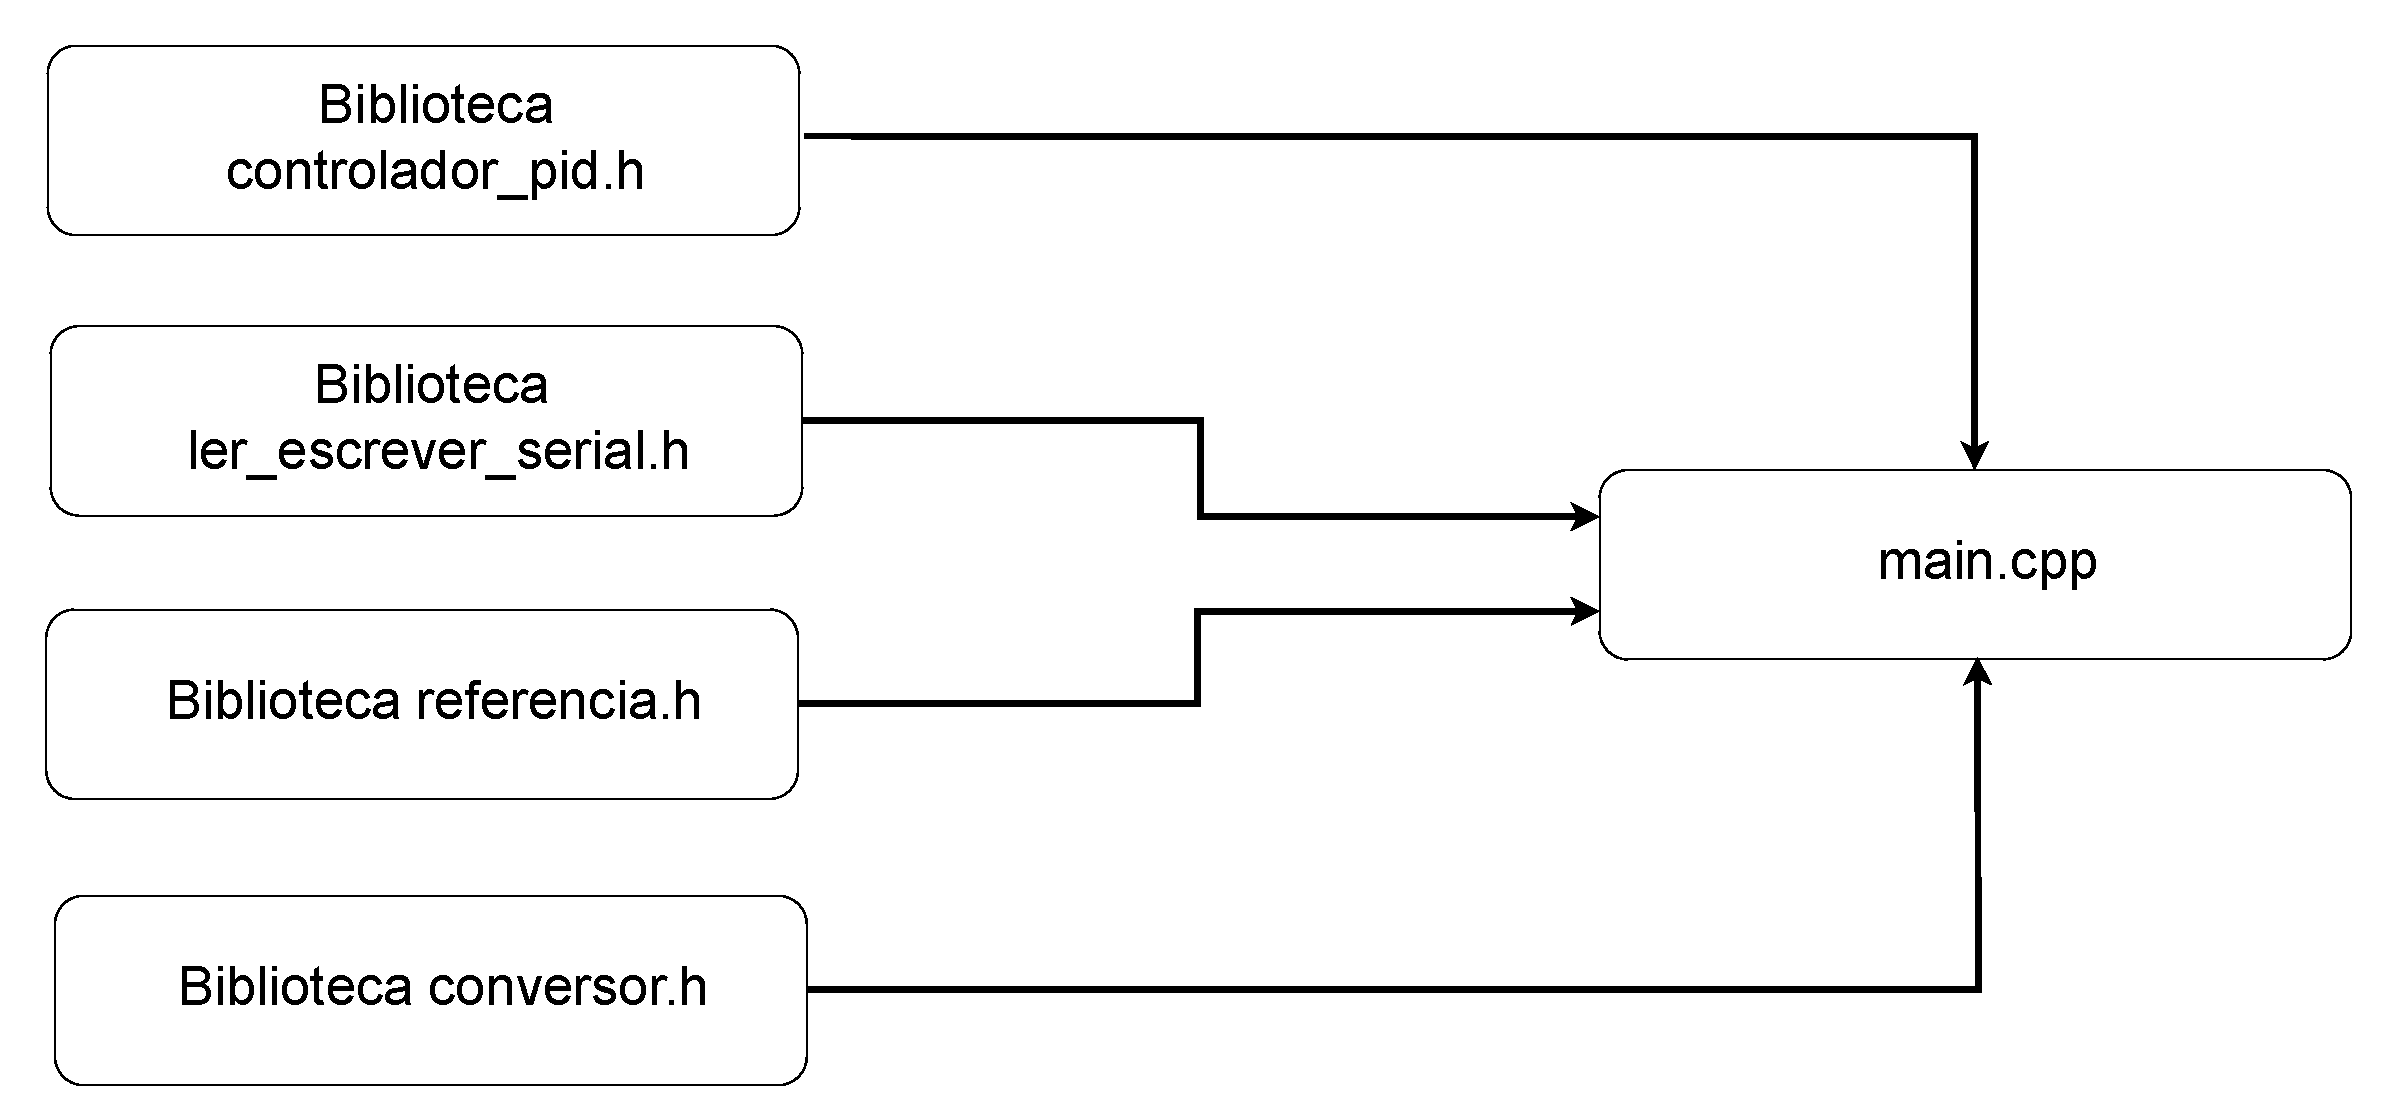
\includegraphics[width=0.8\textwidth]{Capitulos/3_hardware_softwares/3_figuras/arquitetura_firmware.pdf}}
	\caption*{Fonte: elaborado pelo autor (2023).}
	\label{fig3:image_16}
\end{figure}


\subsubsection{Biblioteca ler\_escrever\_serial}

Para realizar a configuração dos parâmetros do sinal de referência em tempo real e o envio dos sinais do sistema via porta serial foi desenvolvido a biblioteca ler\_escrever\_serial, assim, a parte de recebimento e envio de dados do sistema fica centralizada permitindo sua melhoria e modificação sem interferir na lógica do código principal "main.cpp".

\subsubsection{Biblioteca referencia}

O sistema em malha fechada possui uma entrada de referência que o controlador tem por finalidade rastrear, para tornar o projeto do firmware mais legível criou-se o módulo referencia.h em que implementa inicialmente três sinais de referência com a possibilidade de configurar os parâmetros de Amplitude, frequência e offset, sendo esses sinais Onda Quadrada, Onda Senoidal e Onda Dente de Serra. Caso, observe-se a necessidade de outros sinais, basta adicionar a biblioteca.

\subsubsection{Biblioteca conversor}


Essa biblioteca possui uma classe cpp com métodos de conversões de diferentes grandezas, a primeira conversão é do sinal de um potenciômetro para angulo, o segundo método converte o sinal de controle para ciclos PWM, o terceiro método converte de grau para radiano e o quarto de radiano para grau.

\subsubsection{Biblioteca controlador\_pid}

Essa biblioteca implementa uma classe cpp para o controlador PID para ser empregado no protótipo quando selecionado a opção em malha fechada na interface gráfica.


\subsubsection{Arquivo Principal mian.cpp}

A ferramenta PlatformIO possui uma estrutura que permite a criação de bibliotecas e um arquivo main.cpp que implementa a lógica do algorítimo, com isso é possível incluir as bibliotecas desenvolvidas e criar o algorítimo para o que se deseja.


Ou seja, o firmaware para o projeto possui várias funcionalidades que passam pela implementação do sinal de referência, leitura do sensor potenciômetro, envio e recebimento de dados via porta serial e implementação do controlador.

Por fim, com o firmware finalizado, o envio para o ESP32 é realizado usando o PlatfrmIO que concretiza a compilação e escrita no microcontrolador via porta serial.